\section{ХОД РАБОТЫ}

\subsection{Постановка задачи}

Требуется найти вектор градиента и матрицу Гессе для функции $y = z^6 - 2z - 7$,
сделав предварительно подстановку $z = a_1x_1 + a_2x_2$.

Выполнить аппроксимацию функции двух переменных отрезками ряда Тейлора
в окрестности некоторой точки. Отобразить графики функции и аппроксимирующих
полиномов. Проанализировать точность аппроксимации при различном числе
слагаемых ряда Тейлора.


\subsection{Теоретические сведения}
\label{sub:theory}

С помощью векторно-матричного подхода можно записать лишь три члена
ряда Тейлора для скалярной функции $f(X)$ векторной переменной
$X = (x_1, x_2, \dots, x_n)$ в окрестности
точки $X^{(0)} = (x_1^{(0)}, x_2^{(0)}, \dots, x_n^{(0)})$:
\begin{equation*}
  f(X) \approx f(X^{(0)}) + A^T (X-X^{(0)}) + \dfrac{1}{2} (X-X^{(0)})^T B(X-X^{(0)}),
\end{equation*}
где \hspace{1.5mm}  $(X-X^{(0)})^T = ((x_1 - x_1^{(0)}), (x_2 - x_2^{(0)}), \dots, (x_n - x_n^{(0)})), $ \par
                  $A = \dfrac{df}{dX} = (\dfrac{\partial f}{\partial x_i}), i = 1,2,\dots,n$ ---
                  производная функции $f(X)$ \par 
                  в точке $X^{(0)}$, которая называется градиентом функции $f(X)$ в точке~$X^{(0)}$:
\begin{equation*}
  A^T = \bigg( \dfrac{\partial f}{\partial x_1}, \dfrac{\partial f}{\partial x_2}, \dots, \dfrac{\partial f}{\partial x_n} \bigg).
\end{equation*}

Матрицей Гессе называется вторая производная функции $f(X)$ в точке~$X^{(0)}$:
\[
  B =
    \left(
      \begin{array}{cccc}
        \frac{\partial^2}{\partial x_1 \partial x_1} & \frac{\partial^2}{\partial x_1 \partial x_2} & \dots & \frac{\partial^2}{\partial x_1 \partial x_n} \\
        \frac{\partial^2}{\partial x_2 \partial x_1} & \frac{\partial^2}{\partial x_2 \partial x_2} & \dots & \frac{\partial^2}{\partial x_2 \partial x_n} \\
        \dots & \dots & \dots & \dots \\
        \frac{\partial^2}{\partial x_n \partial x_1} & \frac{\partial^2}{\partial x_n \partial x_2} & \dots & \frac{\partial^2}{\partial x_n \partial x_n} \\
      \end{array}
    \right).
\]

Записать последующие члены ряда Тейлора с помощью векторно-матричного подхода в теории
скалярно-матричного дифференцирования не представляется возможным.


\subsection{Получение градиента функции $y(X)$}
\label{subs:gradient}

Построим градиент $A^T$ для функции $y(X) = y(x_1, x_2) = z^6 - 2z - 7$, 
$z = a_1 x_1 + a_2 x_2$. Для этого вычислим производные $\dfrac{\partial y}{\partial x_1}$
и $\dfrac{\partial y}{\partial x_2}$ по правилу нахождения производной сложной функции:
\begin{align*}
  &\frac{\partial y}{\partial x_1} = \frac{\partial y}{\partial z} \cdot \frac{\partial z}{\partial x_1}, 
  &\frac{\partial y}{\partial x_2} &= \frac{\partial y}{\partial z} \cdot \frac{\partial z}{\partial x_2}, \\
  &\frac{\partial z}{\partial x_1} = a_1, \hspace{3cm} \frac{\partial y}{\partial z} = 6z^5 - 2, &\frac{\partial z}{\partial x_2}& = a_2, \\
  &\frac{\partial y}{\partial x_1} = a_1 (6z^5 - 2), &\frac{\partial y}{\partial x_2} &= a_2 (6z^5 - 2).
\end{align*}

В итоге градиент функции $y(X)$ будет иметь вид:
\begin{equation*}
  A^T = \Big( a_1 (6z^5 - 2), a_2 (6z^5 - 2) \Big).
\end{equation*}

\newpage


\subsection{Получение матрицы Гессе функции $y(X)$}

Запишем искомую матрицу Гессе функции $y(X)$ в общем виде:
\[
  B =
    \left(
      \begin{array}{cc}
        \frac{\partial^2 y}{\partial x_1^2} & \frac{\partial^2 y}{\partial x_1 \partial x_2} \\
        \frac{\partial^2 y}{\partial x_2 \partial x_1} & \frac{\partial^2 y}{\partial x_2^2} 
      \end{array}
    \right).
\]

Используя полученные в подразделе~\ref{subs:gradient} выражения, найдём вторые производные
функции $y(X)$, которые будут являться элементами матрицы Гессе:
\begin{align*}
  \frac{\partial y}{\partial x_1} &= \frac{\partial y}{\partial z} \cdot \frac{\partial z}{\partial x_1} = t,
  &\frac{\partial y}{\partial x_2}& = \frac{\partial y}{\partial z} \cdot \frac{\partial z}{\partial x_2} = p, \\
  \frac{\partial^2 y}{\partial x_1^2} &= \frac{\partial t}{\partial x_1} = \frac{\partial t}{\partial z} \cdot \frac{\partial z}{\partial x_1},
  &\frac{\partial^2 y} {\partial x_2^2}& = \frac{\partial p}{\partial x_2} =  \frac{\partial p}{\partial z} \cdot \frac{\partial z}{\partial x_2}, \\ 
  \frac{\partial^2 y}{\partial x_1 \partial x_2} &= \frac{\partial t}{\partial x_2} = \frac{\partial t}{\partial z} \cdot \frac{\partial z}{\partial x_2},
  &\frac{\partial^2 y}{\partial x_2 \partial x_1} &= \frac{\partial p}{\partial x_1} = \frac{\partial p}{\partial z} \cdot \frac{\partial z}{\partial x_1}.
\end{align*}

Таким образом, матрица Гессе будет иметь вид:

\[
  B =
    \left(
      \begin{array}{cc}
        30 z^4 a_1^2 & 30 z^4 a_1 a_2 \\
        30 z^4 a_1 a_2 & 30 z^4 a_2^2 \\
      \end{array}
    \right)
  .
\]

Исходный код разработанной программы приведен в приложении А.


\subsection{Построение графиков}
Выполним аппроксимацию функции двух переменных отрезками ряда Тейлора, используя
векторно-матричный подход.

\newpage

На рисунках~\ref{pic:real}, \ref{pic:taylor} приведены
графики самой функции $y(X)$ и её аппроксимирующего полинома в
окрестности точки $X^{(0)} = (1, 1)$ соответственно.

\begin{figure}[h!]
  \centering
  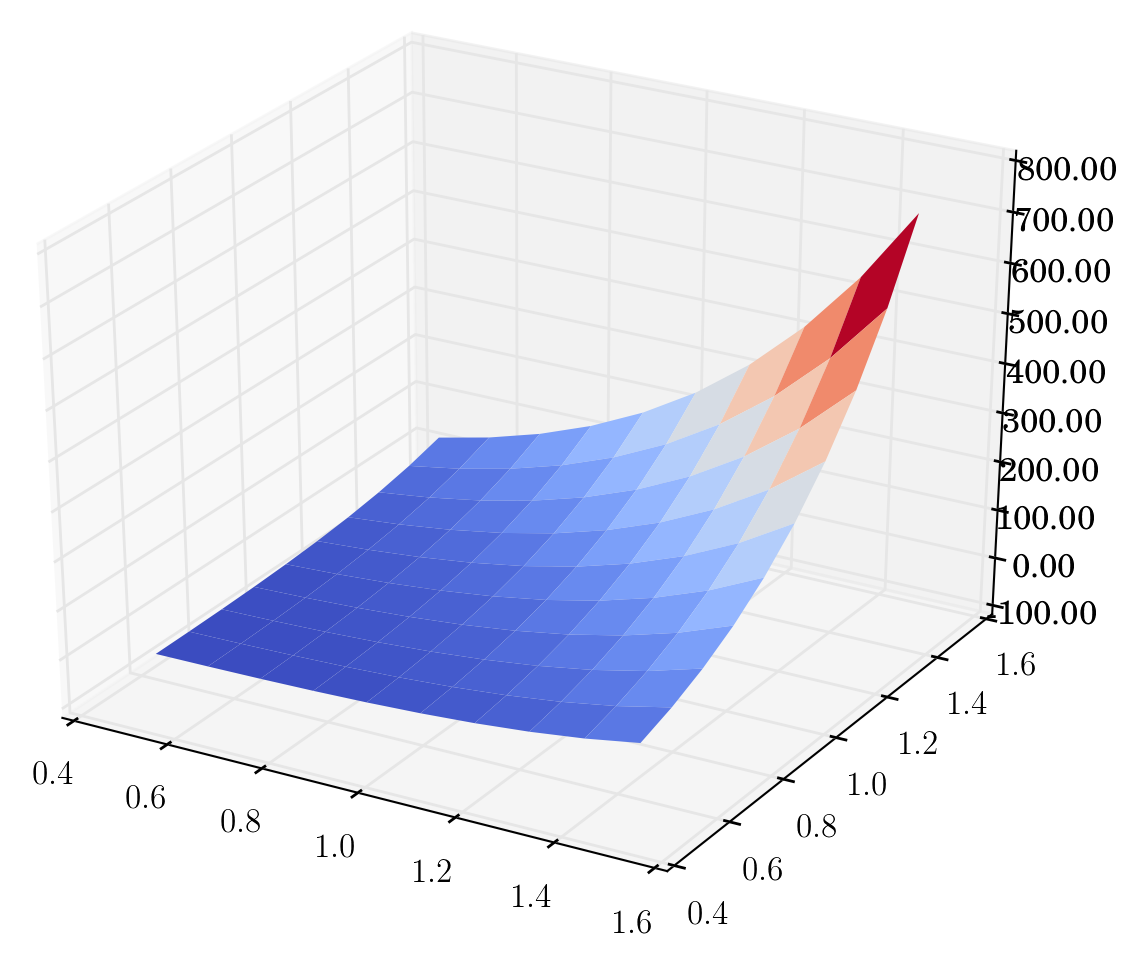
\includegraphics[width=0.65\linewidth]{pic/real_2}
  \caption{График функий $y(X)$}
  \label{pic:real}
\end{figure}

\begin{figure}[h!]
  \centering
  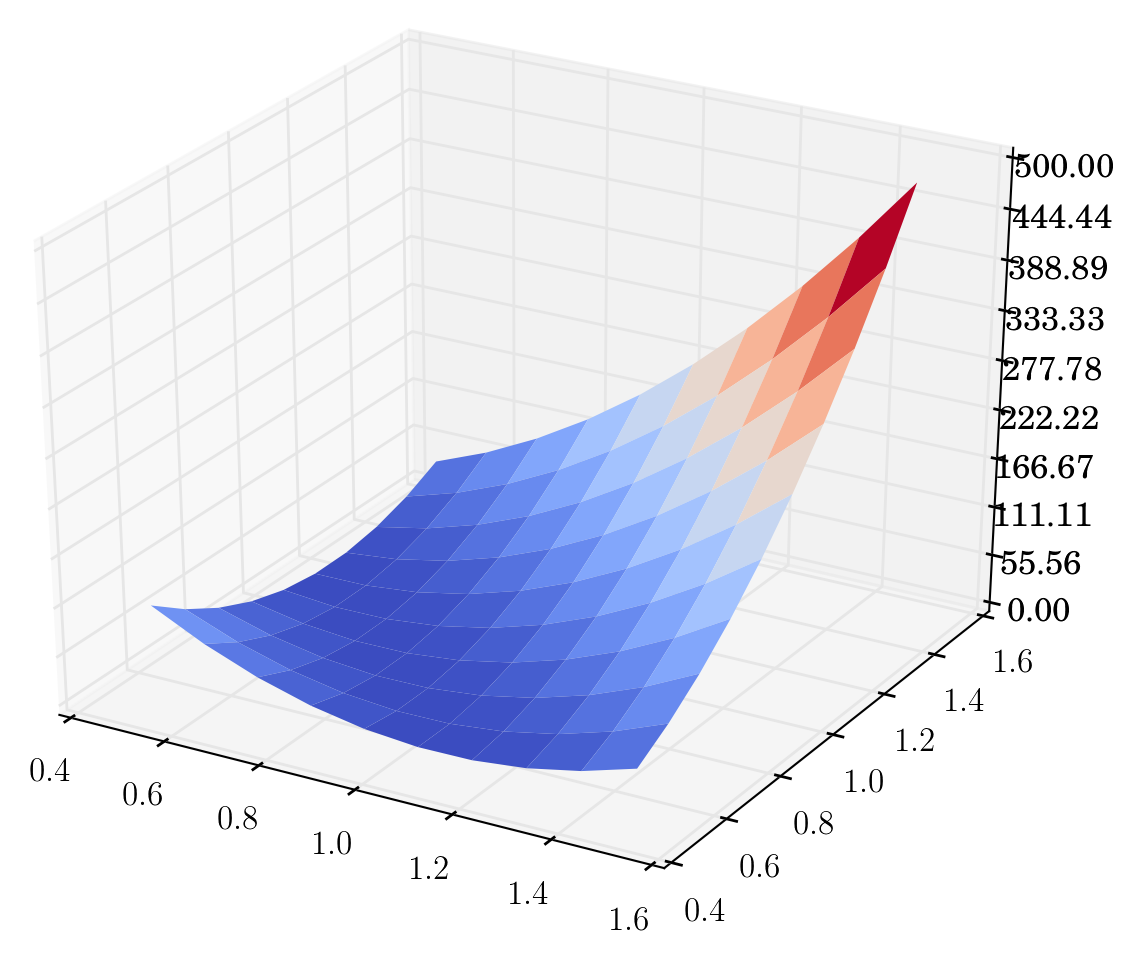
\includegraphics[width=0.65\linewidth]{pic/taylor_2}
  \caption{График аппроксимирующего полинома функции $y(X)$}
  \label{pic:taylor}
\end{figure}
